%-------------------------------------------------------------------------------
% Rules.tex
%-------------------------------------------------------------------------------
% 2024-03-20
% curtis
%-------------------------------------------------------------------------------
% Rules description of TacSubMicro
%-------------------------------------------------------------------------------

\makeatletter
\def\input@path{{../}}
\makeatother
\documentclass[../TacSubMicroRules.tex]{subfiles}

\begin{document}

\section{Players}%
\label{sec:players}

\rulstrong{\gametitle~ is a solitaire game.}
The player controls the nuclear fast attack submarine (SSN) and tasked with sinking the landing helicopter dock (LHD) before the LHD is alerted to the presence of the SSN.
Die rolls and scripted behavior control the opposing surface units.
A game takes between 20 and 45 minutes, largely depending on the player's success.

\section{Abbreviations}%
\label{sec:abbreviations_and_nomenclature}

\rulstrong{These rules use acronyms and abbreviations listed below:}
\begin{description}
    \item[SSN] Nuclear fast attack submarine
    \item[LHD] Landing helicopter dock
    \item[FF] Frigate
    \item[Helo] Helicopter
    \item[\#''] \# inches; for example, 12'' means ``twelve inches''
    \item[1d6] Rolling one six-sided die
    \item[2d6] Rolling two six-sided dice
    \item[CZ] Convergence zone
    \item[DP] Detection point
    \item[ASW] Anti-submarine warfare
\end{description}

\section{Victory and Defeat}%
\label{sec:victory_and_defeat}

\rulstrong{To win the game, the player must sink the LHD, then escape the pursuing surface units.}

\subsection{Victory}%
\label{sub:victory}

\rulstrong{The player wins the game if all three of the following are simultaneously true:}
\begin{itemize}
    \item The LHD has been sunk (\ref{sub:loose_torpedoes}, \ref{rul:torphitship}).
    \item The SSN is 12'' away from the nearest FF.
    \item The SSN was not detected by any surface units during a surface detection step (\ref{rul:surfdetection}).
    \item The SSN leaves the table.
\end{itemize}

\subsection{Defeat}%
\label{sub:defeat}

\rulstrong{The player loses the game if:}
\begin{itemize}
    \item Any surface unit leaves the play area prior to sinking the LHD.
    \item The SSN is sunk.
    \item The SSN has no remaining torpedoes and has not sunk the LHD.
\end{itemize}

\section{Materials and Setup}%
\label{sec:materialssetup}

\rulstrong{Most materials to play \gametitle~ are provided with the game after cutting them out.}

\subsection{Dice}%
\label{sub:external_materials}

The player needs to provide six-sided dice (ideally two) to play \gametitle.
In the rules, these dice are referred to as d6.
\rulstrong{Rolling two dice and summing the number of pips showing is called rolling 2d6, while rolling one die is called rolling 1d6.}
Die rolls are used to determine surface units' movement (\ref{rul:surfmaneuver}) resolve sonar detection (\ref{rul:sonarroll}), resolve torpedo kills (\ref{sub:loose_torpedoes}), and resolve SSN evasion.

\subsection{Tape Measure and Distances}%
\label{sub:tape_measure}

Use a tape measure or yard stick with Imperial units when playing \gametitle.
\rulstrong{When measuring distances between counters, measure between nearest counter edges.}

\subsection{Play Area}%
\label{sub:playarea}

\rulstrong{Play \gametitle~ on a large table top.}
There is no rule on exact dimensions.
Note that the geometry of your table determines the difficulty of \gametitle, as the game ends when either any surface unit leaves the table prior to the SSN sinking the LHD (\ref{sub:defeat}) or when the SSN leaves the play area (\ref{sub:victory}).

\gamerule{rul:leavetable} \rulstrong{If a ship, SSN, or helo makes a maneuver (\ref{sub:maneuver}) that results in the counter leaving the table, remove the counter from the game.}
This event may occur if:
\begin{itemize}
    \item A ship moves in a path, either willingly or unwillingly, that takes the counter off the table (\ref{rul:ssnmaneuver}).
    \item A helo moves to a counter that is not on the table..
\end{itemize}
If a DP needs to be placed off the table, do not place the DP at all, and ignore all detection rolls for that DP (\ref{rul:surfdetection}).

\subsection{Counters}%
\label{sub:counters}

\rulstrong{Cut out all (double-sided) game pieces before play.}

\begin{design}
    In all likelihood, you printed \gametitle~ as a print-and-play game and did not get the game as a postcard.
    You will need to assemble the counters yourself.
    You could fold the paper over a piece of cardboard after gluing the game to the cardboard, then cut out the pieces.
    I cut out sections of the pieces single-sided, glue them to cardboard, slice the cardboard so that I have single-sided pieces glued to cardboard, then glue the two cardboard sides together to get double-sided pieces.
    I prefer to cut large sections with a guillotine cutter, though scissors work fine for cutting out the individual counters once I have strips.
    When I glue the two sides together, I have thicker counters that are more easily handled.
    But do whatever works best for you.
\end{design}

\counterpic{HeloShallow}
\gamerule{rul:helo} A helicopter (helo) is a surface unit, an ASW platforms aboard ships that can search for the SSN and attack it if the SSN is found.
Helos have two sides: shallow (light blue) and deep (dark blue).
After a helo has been launched and has moved to its first search location, the side a helo is on indicates the depth at which the helo listens to the SSN.
When the helo listens at a different depth, flip the helo's counter.
Unlike ships and the SSN, helos do not point in any particular direction, since helos are far more maneuverable than ships or boats.
\rulstrong{Helos start the game aboard ships.}

\begin{design}
    Helos in \gametitle~ use dipping sonars to listen for the SSN.
    The helo starts listening at shallow depth.
    As the dipping sonar lowers deeper into the ocean, the helo counter flips over to the deep side to indicate it is now listening for the SSN at a deeper depth.
    After the helo moves, the cycle starts over.
    No, I do not know at what speed a dipping sonar rises or drops in real life, and I chose not to ask (see the design notes for why).
\end{design}

\gamerule{rul:ships} FFs and the LHD are ships.
The SSN is \emph{not} a ship.
Ship counters have two sides: unalerted (light blue) and alerted (red).
\rulstrong{All ships start the game unalerted, so ship counters set up on their unalerted side.}
Ship counters also have an arrow in front of the bow of the ship, indicating the direction the ship points and thus which direction is straight ahead.
When a ship detects the SSN, the ship becomes alerted; flip the ship counter over to the alerted side.
Ships always listen for the SSN at shallow depth (\ref{rul:sonarthreshold}).
Die rolls determine ship maneuvers, with all ships making identical maneuvers if the LHD is sailing, or FFs moving towards the SSN if the LHD is sunk.
When a ship launches a helo, leave the helo at the ship's old position, move the ship, then move the helo according to the helo's maneuver rules.

\begin{design}
    SSNs are not ships.
    This is not just for rules convenience; in the US Navy, SSNs are called ``boats.''
    Not only is this a historical term, it also fits with a technical definition the US Navy uses differentiating ships from boats.
    The center of mass on a ship is at higher altitude on a ship's hull, and results in a ship turning away from the direction in which the ship is turning.
    Boats have a lower center of mass and turn into the direction they are turning.
    By this definition, FFs and LHDs are ships and SSNs are boats, despite the size of a SSN or even a SSBN (a nuclear ballistic missile submarine).
\end{design}

\widecounterpic{FFUnalert}
\gamerule{rul:ff} A frigate (FF) is a ship that escorts the LHD.
\rulstrong{Place four FFs in the play area such that they form a square with 4'' separating each FF, all pointing in the same direction, and with one helo (on its shallow side) aboard each FF.}

\widecounterpic{LHDUnalert}
\gamerule{rul:lhd} The LHD is the SSN's target; it must be sunk for the SSN to win the game (\ref{sub:victory}).
\rulstrong{Place the LHD in the center of the FF square equidistant from all four FFs, pointing in the same direction, and with two helos (on their shallow side) aboard.}

\widecounterpic{SSNDeep}
\gamerule{rul:ssn} The player controls the nuclear fast attack submarine (SSN) counter (\ref{sec:players}).
The counter has two sides, shallow (dark blue) and deep (light blue).
Like ships, the SSN has an arrow at the front of its counter before the SSN's bow indicating its direction of travel and what is straight ahead of the SSN.
\rulstrong{Place the SSN in the play area 30'' away from the nearest FF on its deep depth side.}
When the SSN changes depth, flip its counter to the appropriate side.

\begin{design}
    As discussed in \ref{sub:playarea}, the geometry of the play area and player setup determines \gametitle's difficulty.
    The setup rules above do not give a unique setup configuration.
    I encourage players to experiment with different play areas and SSN positions relative to the surface units.
    See how difficult different configurations are.
    If the SSN is directly behind a surface group about to leave the play area, the game will be quite difficult.
    On the other hand, if the SSN is sitting right in front of a surface group with plenty of space between table edges, the SSN may have a much easier time.
    This latter setup treats the SSN like a ``mobile minefield,'' a concept of operations used by diesel-electric submarines (SSKs) that take advantage of SSK's silence when running on their batteries, but this tactic is available to SSNs as well.
\end{design}

\counterpic{DP2S}
\gamerule{rul:dp} As the SSN moves through the play area, the player places detection point (DP) counters that surface units use during their sonar detection roll (\ref{rul:surfdetection}) and FFs or helos move toward when pursuing the SSN.
The game provides six double-sided DP counters, of which only three will be on the table (except at the start of the game prior to the SSN taking its first turn).
On each counter is a number from one to three and, on each side of the counter, a letter corresponding to speed levels of the SSN: (C)reep, (S)low, (F)ast, and f(L)ank.
(Creep and slow share a counter, fast and flank a different counter.)
The number on the counter matters only for when helos or FFs need to decide in which direction to travel, and all that matters is that all three numbers be placed on the table after the SSN finishes its maneuver (\ref{rul:ssnmaneuver}); in other words, the player is not obligated to place the DP numbers in any particular order.
However, the speed level indicated by the DP counter matters, and is determined during the SSN's maneuver step.
One DP will be beside the SSN, while the other two will be away from the SSN.
The two DPs away from the SSN will be accompanied by depth counters that show the depth of the DP, while the depth of the DP beside the SSN is determine by the depth of the SSN.
\rulstrong{Place any slow DP (any number) beside the SSN after placing the SSN in the play area during game setup; note that this means that the SSN starts the game having traveled slow (which means the SSN's next maneuver cannot be at flank speed).}

\begin{design}
    I use DPs to model uncertainty about the SSN's position in the play area.
    They help mitigate dynamics I fear may emerge by a IGO-UGO ruleset.
    Additionally, helos and FFs need to move toward the SSN, but they are uncertain about the SSN's position, so I have them go to a random DP as a part of their search pattern.
\end{design}

\gamerule{rul:torpkill} \rulstrong{Torpedo counters track torpedo movement when units loose torpedoes (\ref{rul:torphoming}) and flip over to their kill side (with a skull and crossbones) when a torpedo achieves a kill (\ref{rul:torphitship}).}
\begin{wrapfigure}{r}{25.4mm}
    \centering
    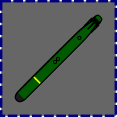
\includegraphics[width=10.7mm]{HeavyTorp}
    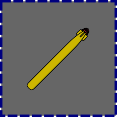
\includegraphics[width=10.7mm]{LightTorp}
\end{wrapfigure}
The SSN begins the game with four heavyweight torpedoes (green); after a torpedo is loosed, it either marks a kill or is removed from the game.
Ships and helos share a lightweight torpedo (yellow) counter that can be reused.
When the SSN runs out of torpedo counters, the SSN can no longer loose torpedoes; if the SSN has not sunk the LHD with four torpedoes, the SSN loses the game (\ref{sub:defeat}).

\begin{design}
    I often prefer to move the SSN with its torpedoes stacked on or near the SSN counter, but this is not required.
\end{design}

\gamerule{rul:dcmarker} \rulstrong{When the SSN wishes to change depth, the player places the depth change counter beside the SSN during the SSN's maneuver step (\ref{rul:ssnmaneuver}).}
\counterpic{Rise}
If the SSN wishes to change from deep to shallow, the player places the counter on the rise side.
If the SSN wishes to change from shallow to deep, the player places the counter on the dive side.
The player may place the counter after the SSN finishes its movement.
The SSN cannot place the depth change marker if the SSN loosed torpedoes that turn (\ref{sub:loose_torpedoes}).
The depth change marker will determine the depth of the DP placed in front of the  SSN (\ref{rul:ssnmaneuver}).

\counterpic{DepthDeep}
\gamerule{rul:dpdepth} Depth counters have a deep side (dark blue) and a shallow side (light blue).
\rulstrong{Place a depth counter corresponding to SSN's current depth (prior to changing the SSN's depth, as indicated by the presence of the depth change counter) beside the DP currently beside the SSN when the SSN begins its maneuver step (\ref{rul:ssnmaneuver}); then, after the SSN finishes its movement and has decided whether to place a depth change counter beside it, place a depth counter beside the DP placed in front of the SSN corresponding to the depth the SSN will have at the end of its next maneuver step.}
The depth marker beside a DP determines the DP's depth, which affects sonar detection rolls (\ref{sub:detection_rolls}).
\gametitle~ uses two depth markers, since the depth of the DP beside the SSN is determined by the SSN counter.

\subsection{Turn Tool}%
\label{sub:turn_tool}

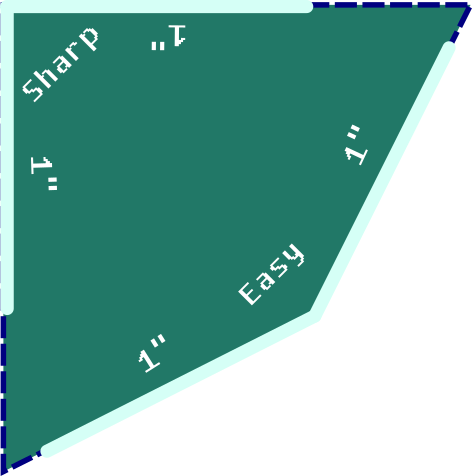
\includegraphics[width=1.0\linewidth]{TurnTool}
\gametitle~ provides a turn tool for whenever a ship (\ref{rul:ships}) or the SSN (\ref{rul:ssn}) need or wish to make a turn.
One corner of the turn tool is labeled ``Easy'' and the other ``Sharp.''
The maneuvering counter uses one of these two corners when making a turn.
These corners determine the tightest angle at which a ship can turn.
Which corner a unit can use depends on the unit's speed (\ref{sub:maneuver}; note that ships always use the easy corner).
The turn tool also has light-colored regions useful for measuring distances.
The length of the light-colored region is 1'' (if the turn tool was printed at the right scale).
\rulstrong{When using the turn tool, place the corner of the turn tool being used so it touches the front (bow) corner of the maneuvering counter on the side of the counter that the counter is turning towards, possibly so that the side of the turn tool is flush with the side of the counter (but this is not required, in case a shallower turn is desired); then, place the maneuvering counter so that it is flush with the turn tool and at the end of the 1'' region on the turn tool ahead of the counter.}
Moving towards the end of the turn tool counts as part of the distance the counter travels.
Note that counters must travel a minimum distance before they can use the turn tool, with that minimum distance determined by the counter's speed.
See Figure \ref{fig:TurnIllustration} for an illustration on using the turn tool.

\begin{design}
    While \gametitle~ requires a measuring tape or ruler to play, players often find that the turn tool does a good job at stepping out the movement of ships and the SSN.
    For example, they will place the SSN right before the 1'' space on the sharp side of the turn tool, then move the SSN to the end of the 1'' space, thus moving the SSN 1'' forward.
    This can be handy if a counter needs to make multiple turns as part of its maneuver step, as the turn tool can help measure out the mandatory intermediate forward movements between turns.
\end{design}

\begin{Figure}
    \centering
    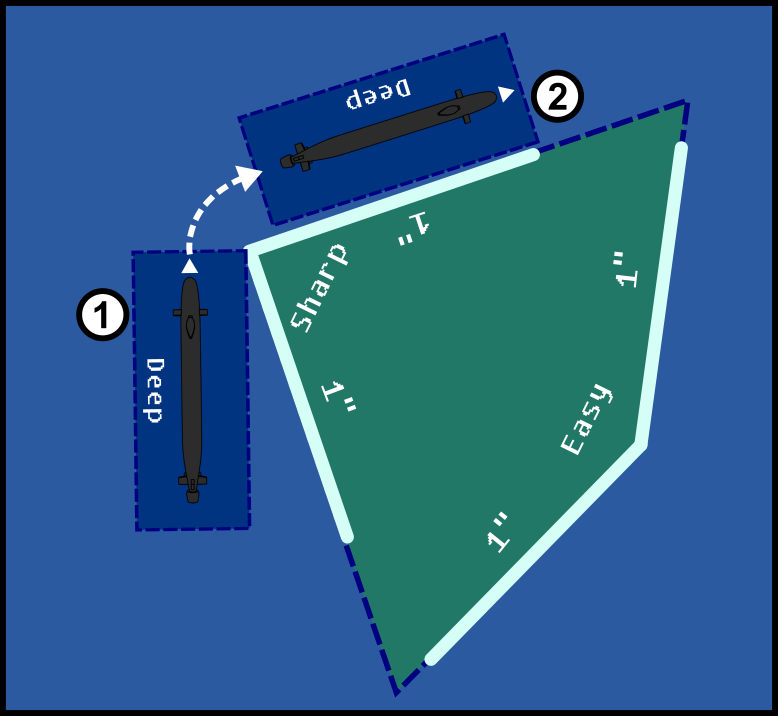
\includegraphics[width=1.0\linewidth]{TurnIllustration}
    \captionof{figure}{The SSN is travelling at slow speed and, during its maneuver step, wishes to make a turn to the right (starboard).
                       The SSN can make a sharp turn, but the player does not want the SSN to make the complete 90° turn.
                       If the player did want the SSN to make a 90° turn, the player would have placed the turn tool so that the corners of the counter and the turn tool touched on the SSN's starboard side and with the turn tool was flush in the counter.
                       But instead, the SSN has the turn tool touch only the corner and turns it slightly so that the SSN makes a more shallow turn (1).
                       Once the turn tool has been placed, the player moves the SSN to the end of the 1'' space marked on the turn tool in front of the SSN, with the SSN counter ending flush with the turn tool (2).}
    \label{fig:TurnIllustration}
\end{Figure}

\section{Sequence of Play}%
\label{sec:sequence_of_play}

\rulstrong{Starting with the SSN, play alternates between the (player-controlled) SSN and (dice-controlled) surface units completing the following steps during their turn:}
\begin{enumerate}
    \item Roll to detect the SSN (surface units only; \ref{sub:surface_detection_step}).
    \item Loose torpedoes (\ref{sub:loose_torpedoes}).
    \item Maneuver (\ref{sub:maneuver}).
\end{enumerate}

\begin{design}
    If you have any real-world experience with undersea warfare, you will likely notice things while playing \gametitle~ and say, ``Wait a minute, that's not right!''
    Early on when designing my tactical submarine games, I decided not to ever ask questions related to key performance parameters of the platforms and weapons I was depicting.
    Such parameters include ranges, speeds, dipping rates, and so on.
    I did not want someone to perceive me as saying something I should not say, especially when the end goal was to post a complete game as a PNG on Twitter without asking for anyone's consent to me doing so.
    As a result, some things do not line up with reality.
    I may do things differently if I revisit this design, but only if I expect to be paid.
\end{design}

\subsection{Detection Rolls}%
\label{sub:detection_rolls}

\rulstrong{Detection rolls occur when the surface units (ships and helos) listen for the SSN using its passive sonar at the start of their turn, or during torpedo attacks, with the torpedo using active sonar to home on its target.}

\gamerule{rul:sonarthreshold} \rulstrong{The sonar detection threshold starts at 19, then the player subtracts modifiers from the starting number to determine the final threshold that the die roll must exceed.}
Every detection roll consists of two parties: a listener, and a target.
During surface detection rolls in the surface detection step (\ref{sub:surface_detection_step}), the listener is a ship or helo, and the target is a DP.
During torpedo attack detection rolls (\ref{rul:torphoming}), the listener is the active torpedo and the target is the target ship or SSN the torpedo is homing on (\emph{not} a DP).
The listener is either at shallow or deep depth.
Ships always listen at shallow depth, while other counters may vary the listening depth.
Similarly, the target is either at shallow or deep depth.
If the listener is at shallow depth, the target must be within a CZ in order for detection to be possible; otherwise, the detection roll automatically fails (though the roll is still considered to have taken place, even if the player does not physically roll the dice).
The listener is either using passive sonar or active sonar, with passive sonar used by unalerted ships, and active sonar used by alerted ships, helos, and torpedoes.
Some modifiers depend on which sonar type the listener is using.
See Table \ref{tab:detection} for a full list of modifiers to the detection threshold possible.
Note that it's possible for a final threshold value to exceed 12, in which case detection is not possible and the player may skip rolling the dice, though the roll is still considered to have happened (which may matter during torpedo attacks targeting the SSN).

\begin{Table}
    \centering
    \captionof{table}{Detection threshold computation}
    \begin{tabular}{R{0.65\linewidth}|L{0.15\linewidth}}
        \hline
        \hline
        \dtabsec{All}
        \dtabrow{Starting Threshold}{$\ge 19$}
        \dtabrow{Listener Shallow, No CZ}{Fail}
        \dtabrow{Target Same Depth}{$-3$}
        \dtabrow{Target Ship, SSN, or DP Beside SSN}{$-3$}
        \hline
        \dtabsec{Active Sonar}
        \dtabrow{Listener Shallow, CZ}{$-8$}
        \dtabrow{Listener Deep}{$-6$}
        \dtabrow{Target Is a Ship}{$-3$}
        \hline
        \dtabsec{PASSIVE SONAR}
        \dtabrow{Target Speed is Creep}{$-2$}
        \dtabrow{Target Speed is Slow}{$-4$}
        \dtabrow{Target Speed is Fast}{$-6$}
        \dtabrow{Target Speed is Flank}{$-8$}
        \dtabrow{Listener Shallow, CZ}{$-2$}
        \dtabrow{Listener Deep}{$-2$}
        \hline
    \end{tabular}
    \label{tab:detection}
\end{Table}

\gamerule{rul:cz} A convergence zone (CZ) is a region where a target must be present in order for a listener at shallow depth to be able to detect the target.
CZs repeat with distance; there is no limit to the number of CZs around a listener.
\rulstrong{CZs start 4'' away from the listener, each spans 4'', and each is separated from another CZ by 4''.}
For example the first CZ is a ring around the listener from 4''away from the listener to 8'' away, the second CZ is a ring starting 12'' away and ending 16'' away, and so on.
If any part of a target's counter is inside a CZ, the target is considered to be inside the CZ.
See Figure \ref{fig:CZIllustration} for an illustration.

\begin{Figure}
    \centering
    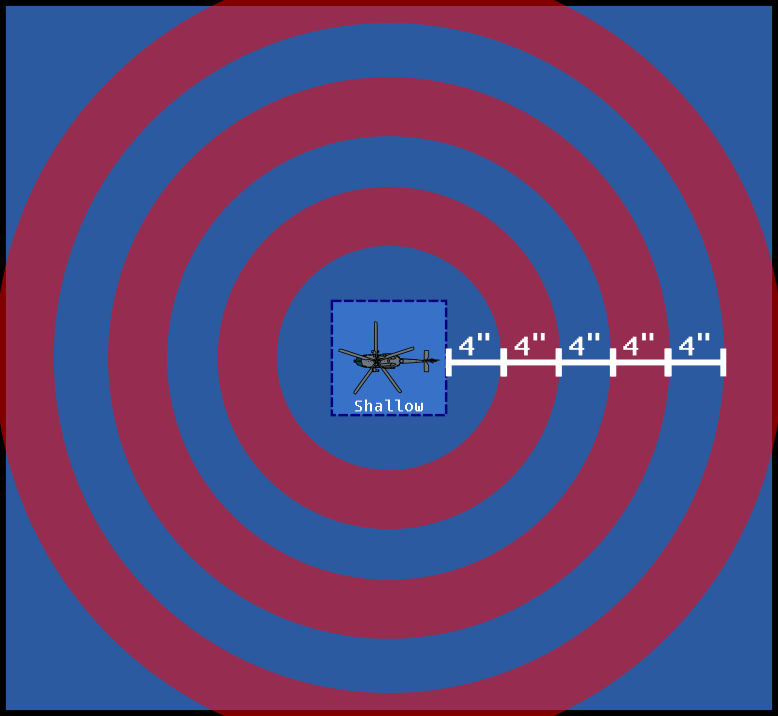
\includegraphics[width=1.0\linewidth]{CZIllustration}
    \captionof{figure}{Illustration of three CZs surrounding a listening helo at shallow depth (not drawn to scale).
                       A CZ is shaded red.
                       If the helo were listening for the SSN using active sonar, the SSN must be within one of the CZs to be detectable.}
    \label{fig:CZIllustration}
\end{Figure}

\gamerule{rul:sonarroll} \rulstrong{To make a detection roll, roll 2d6; the detection roll succeeds if the sum is equal to or greater than the detection threshold.}
In some cases a successful detection may not be possible, in which case the player may forgo rolling the dice.
The roll is still considered to have happened even if it automatically failed.
See \ref{fig:DetectIllustration} for an example.

\begin{Figure}
    \centering
    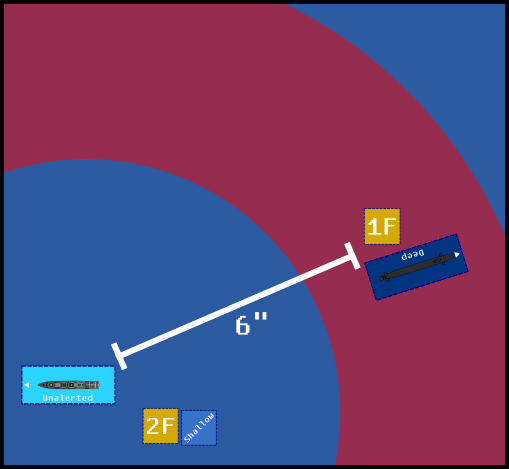
\includegraphics[width=1.0\linewidth]{DetectIllustration}
    \captionof{figure}{In this example (not drawn to scale), a FF listens for the DP beside the SSN during the surface detection step (\ref{sub:surface_detection_step}) at shallow depth using active sonar.
                       CZs affect the FF's ability to detect the SSN due to listening at shallow depth; since the DP is 6'' away and thus within a CZ (which spans from 4'' away from the FF to 8'' away), the FF might be able to detect the SSN.
                       When computing the detection threshold for whether the FF can detect the DP, the player starts with the starting threshold of 19.
                       DP 1 is within a CZ (unlike DP 2) and thus might not have an automatically failed detection roll.
                       Since the depth of the DP is deep (since the DP is beside the SSN and the SSN's depth is deep), the player does not apply the $-3$ modifier for the target being at the same depth as the listener.
                       However, DP 1 is beside the SSN (unlike DP 2) and thus the player applies a $-3$ modifier to the threshold, bringing it down to 16.
                       Next, the player looks to the passive sonar rows of the detection table (Table \ref{tab:detection}).
                       The speed indicated by the DP is fast, so the player applies the $-6$ modifier to the detection threshold, bringing it down to 10.
                       Since the listener is at shallow depth and the target is inside a CZ, the player applies another $-2$ modifier; the final detection threshold is 8.
                       The player rolls 2d6 and gets 7, a failed detection since it is less than the detection threshold.}
    \label{fig:DetectIllustration}
\end{Figure}

\begin{design}
    In the example in Figure \ref{fig:DetectIllustration}, the convergence zone is measured starting from the FF and going to the DP.
    Measuring distance starting from the DP and going to the FF also works (since the distance from point A to point B is the same as the distance from point B to point A).
    I prefer to measure distance starting at DPs during the surface detection step (\ref{sub:surface_detection_step}) since I prefer to compute a worst-case-scenario detection threshold for the DP, roll the dice, then determine which surface units were in range to successfully detect.
    This works best when measuring distance starting from the DP and going to the surface units.
\end{design}

\subsection{Surface Detection Step}%
\label{sub:surface_detection_step}

During the surface detection step, surface units listen for the SSN, and react accordingly.
The surface detection step happens before attacks and maneuvers for surface units.
One of two outcomes can result from successful surface detection of the SSN:
\begin{itemize}
    \item Unalerted ships become alerted, which results in ships using active sonar and potentially attacking the SSN.
    \item Alerted units (helos are always alert) attack the SSN during the surface units' loose torpedoes step (\ref{sub:loose_torpedoes}).
\end{itemize}
\rulstrong{The surface detection step consists of two substeps:}
\begin{enumerate}
    \item Spread alertment (\ref{rul:detectspread}).
    \item Make detection rolls for each DP (\ref{rul:surfdetection}).
\end{enumerate}

\gamerule{rul:detectspread} \rulstrong{If any ship started the surface detection step alerted and unalerted ships remain, alert all unalerted ships.}
Note that the newly alerted ships did not start the SSN's step alerted, so they will not launch helos this turn.

\gamerule{rul:surfdetection} \rulstrong{Make a detection roll (\ref{sub:detection_rolls}) for each DP in the play area.}
Roll 2d6 once for each DP; each surface unit determines independently whether the result of the die roll results in a successful detection (different surface units likely have different detection thresholds).
Ships always listen at shallow depth.
Helos listen at the depth shown on their counter if they have not launched from their ship this turn.
Unalerted ships use passive sonar.
Helos and alerted ships use active sonar.
Remember that if the SSN is at least 12'' away from the nearest FF after sinking the LHD and is not detected during this step, the SSN wins the game (\ref{sub:victory}).

\begin{design}
    During this step, I use the sonar detection table (Table \ref{tab:detection}) to determine what the most likely detection scenario is.
    Then, I make the detection roll, and figure out for which ships the roll is a successful detection after the roll is over.
    This can get tricky when helos listen at different depths, and I just need to remember that I need to handle helos listening at deep depth separately.
\end{design}

\gamerule{rul:surfdetectresults} \rulstrong{Successful detection rolls for unalerted ships (\ref{rul:ships}) results in the ships becoming alerted (flipping over their counter), while successful detection rolls for helos and alerted ships may result in attacks.}
If a helo or alerted ship is within 12'' of the detected DP, it will loose one or two torpedoes during the surface units' loose torpedoes step (\ref{sub:loose_torpedoes}).
(The torpedo will target the SSN and is still subject to the 18'' fuel range rule.
A helo or alerted ship that was not within 12'' of the ship does nothing.)

\subsection{Loose Torpedoes}%
\label{sub:loose_torpedoes}

Surface units may loose torpedoes at the SSN if they detected the SSN using active sonar (\ref{rul:surfdetection}) during the surface units' detection step,
The SSN may loose torpedoes at a ship (\ref{rul:ships}) at the start of its turn.
Multiple torpedoes may be launched in a turn; resolve each attack separately.
Torpedo attacks involve a shooter (the counter loosing the torpedo) and a target (where the torpedo will go and the counter that may be sunk if the attack is successful).
\rulstrong{Resolving a torpedo attack requires:}
\begin{enumerate}
    \item Loosing the torpedo (\ref{rul:torploose}).
    \item Homing the torpedo onto its target (\ref{rul:torphoming}).
    \item Determining if the torpedo successfully killed its target (\ref{rul:torphitship}, \ref{rul:torphitssn}).
\end{enumerate}

\gamerule{rul:torploosecount} \rulstrong{Different units fire a different number of torpedoes a turn.}
The SSN can loose at most two torpedoes a turn, at player discretion.
If no SSN torpedo counters remain, the SSN cannot loose torpedoes.
(If the SSN has no torpedoes and the LHD has not been sunk, the SSN loses the game; \ref{sub:defeat}.)
Helos loose two torpedoes, then are removed from the game.
Ships loose one torpedo a turn each.
This is summarized in Table \ref{tab:torploosecount}.
\begin{Table}
    \centering
    \captionof{table}{Torpedoes loosed per turn}
    \begin{tabular}{R{0.15\linewidth}|L{0.65\linewidth}}
        \hline
        \ttabhead{Unit}{Torpedoes Fired}
        \hline
        \hline
        \ttabrow{SSN}{$\le 2$}
        \ttabrow{Ship}{$1$}
        \ttabrow{Helo}{$2$, remove helo from the game}
        \hline
    \end{tabular}
    \label{tab:torploosecount}
\end{Table}

\begin{design}
    Presumably a helo has loosed all its torpedoes and must return to a ship, in which case the game no longer tracks the helo.
\end{design}

\gamerule{rul:torpalert} \rulstrong{Loosing a torpedo alerts all ships immediately.}
Note, though, that ships alerted this way by the SSN loosing torpedoes did not start the SSN's turn alerted.
(Thus, they might not launch helos during the surface units' next turn.)

\gamerule{rul:torprange} \rulstrong{The fuel range of all torpedoes in \gametitle~ is 18''.}
If a target is not within the torpedo's fuel range, the torpedo automatically misses.

\gamerule{rul:torploose} \rulstrong{At the start of a torpedo attack, the torpedo looses at the shooter's depth.}
All surface units loose torpedoes at shallow depth.
Place a torpedo counter at the shooter's location.

\gamerule{rul:torphoming} \rulstrong{Repeat the following torpedo homing process until the torpedo reaches its target:}
\begin{enumerate}
    \item Make a detection roll using the torpedo's active sonar (\ref{sub:detection_rolls}) against the torpedo's target.
        Note the result.
    \item Move the torpedo 5'' in a straight line to its target, or until the torpedo counter reaches the target's counter.
        If the torpedo completed a 5'' move, it is now at the target's depth.
        If the torpedo counter did not start at the target's depth and did not complete a 5'' move, the torpedo misses its target.
\end{enumerate}
The homing process ends when:
\begin{itemize}
    \item The torpedo fails two detection rolls in a row; the torpedo missed the target.
    \item The torpedo reaches its target; if the torpedo is at the target's depth and had at least one successful sonar detection roll while homing, the torpedo hit its target.
\end{itemize}
If one of the SSN's torpedoes missed its target, remove the torpedo counter from the game.
See Figure \ref{fig:TorpAttackIllustration} for an illustration.

\counterpic{Kill}
\gamerule{rul:torphitship} \rulstrong{If a torpedo hit a ship, roll 1d6; on a roll of $2$ or more, flip the torpedo over to its kill side and place it on the ship, marking a kill.}
Otherwise, the torpedo failed to damage the ship sufficiently and is removed from the game.
One torpedo kill sinks a FF, turning the FF into a wreck.
Two torpedo kill shots sinks the LHD, turning the LHD into a wreck (an important part of the SSN winning the game; \ref{sub:victory}).
If the LHD has only one kill on it, the LHD is damaged but not sunk, affecting its maneuvers.

\begin{Figure}
    \centering
    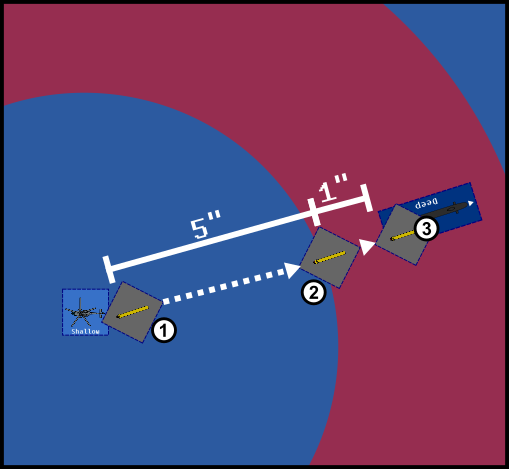
\includegraphics[width=1.0\linewidth]{TorpAttackIllustration}
    \captionof{figure}{A helo detected a DP during the surface units' detection step (\ref{rul:surfdetectresults}), so during the surface units' attack step, the helo attacks the SSN with torpedoes.i
                       The helo will loose two torpedoes, then be removed from the game (\ref{rul:torploosecount}).
                       The SSN is 6'' away and at deep depth.
                       Both of the helo's torpedoes, when loosed, start out at shallow depth (\ref{rul:torploose}).
                       The first torpedo starts homing after being loosed (\ref{rul:torphoming}).
                       Since the torpedo uses active sonar, is at shallow depth, targeting the SSN at deep depth (so not the same depth as the torpedo), and the SSN is in a convergence zone (\ref{rul:cz}), the initial sonar detection threshold is 5 (\ref{rul:sonarthreshold}) (1).
                       The player rolls 2d6 and gets a roll of 4, a failed detection (\ref{rul:sonarroll}).
                       Regardless, the torpedo advances 5'' closer to the SSN in a straight line from its previous position, then makes another detection roll (2).
                       The torpedo is now at the target's depth, deep.
                       Since the torpedo is now at deep depth and the same depth as its target, the new detection threshold is 7.
                       The torpedo rolls 8, a successful detection roll.
                       Thus, the torpedo has not had two failed detection rolls in a row and at least one successful detection, so it moves 1'' to hit the submarine (3).
                       Since the torpedo made two detection rolls, the torpedo's evasion save threshold is 4 (\ref{rul:torphitssn}).
                       With a roll of 5 on 1d6, the SSN successfully evades the torpedo.
                       The helo then drops its second torpedo (which starts homing on the SSN) and is removed from the game.}
    \label{fig:TorpAttackIllustration}
\end{Figure}

\gamerule{rul:torphitssn} \rulstrong{If a torpedo hits the SSN, the SSN first gets an evasion save, with the threshold for success being 6 \emph{minus the number of detection rolls the torpedo made while homing}; if a roll of 1d6 exceeds the threshold, the SSN successfully evaded the torpedo, but otherwise the torpedo killed and sunk the SSN.}
Needless to say, the SSN loses the game if sunk (\ref{sub:defeat})

\begin{design}
    I confess to using the terms ``hit'', ``kill'', and ``sunk'' loosely, and I beg the reader's forgiveness.
\end{design}

\subsection{Maneuver}%
\label{sub:maneuver}

\rulstrong{Both the surface units and the SSN maneuver as the last step of their turns.}
SSN maneuvers are controlled by the player while surface unit maneuvers are determined by die rolls.

\gamerule{rul:ssnmaneuver} \rulstrong{The SSN's maneuver step consists of completing the following steps:}
\begin{enumerate}
    \item Remove all DPs (\ref{rul:dp}) and accompanying depth counters (\ref{rul:dpdepth}) \emph{except for the DP beside the SSN.}
      Place a depth counter beside the DP beside the SSN corresponding to the SSN's current depth.
    \item If a depth change counter (\ref{rul:dcmarker}) is beside the SSN, flip the SSN counter (\ref{rul:ssn}) to the appropriate depth, either to deep if the depth change counter is on its ``dive'' side, or shallow if the depth change counter is on its ``rise'' side.
      Remove the depth change counter.
    \item Move the SSN a number of inches determined by its speed level.
      The speed the SSN travelled last turn is shown on the DP currently beside the SSN.
      The SSN may travel at either the same speed, one level slower (if possible), or one level faster (if possible).
      See Table \ref{tab:speed} for movement rates. 
      The SSN may use the turn tool to turn while it moves (\ref{sub:turn_tool}) with each turn separated by either 1'' at creep or slow speeds, or 2'' at fast or flank speeds.
      This also means that the SSN is required to move 1'' at creep or slow speed, or 2'' at fast or flank speed, before it can use the turn tool for the first time during its maneuver step, and it must complete the post-turn 1'' move as part of using the turn tool.
      All inches moved while using the turn tool count against the total number of inches moved during the SSN's maneuver step.
    \item If the SSN did not loose torpedoes this turn (\ref{rul:torploose}), the SSN may place the dive or rise counter so that it will change its depth \emph{next turn.}
    \item Place any DP beside the SSN.
      Then, place a DP in a straight line in front of the SSN at a distance equal to the distance the SSN traveled this turn.
      The DP must have the speed corresponding to the distance traveled by the SSN this turn.
      Place a depth counter beside that DP as well, corresponding to the depth the SSN will be at when it maneuvers next turn (which may not be the SSN's current depth if there is a depth change counter beside the SSN).
      If a DP cannot be placed in the play area (\ref{sub:playarea}) ahead of the SSN according to the rules above, do not place that DP.
\end{enumerate}
\begin{Table}
    \centering
    \captionof{table}{Submarine speed levels and effects}
    \begin{tabular}{R{0.25\linewidth}|C{0.2\linewidth}|L{0.35\linewidth}}
        \hline
        \stabhead{Speed (Level)}{Inches Moved}{Turning}
        \hline
        \hline
        \stabrow{Creep (1)}{$0$---$2$}{Sharp every 1''}
        \stabrow{Slow (2)}{$>2$---$4$}{Sharp every 1''}
        \stabrow{Fast (3)}{$>4$---$6$}{Easy every 2''}
        \stabrow{Flank (4)}{$>6$---$8$}{Easy every 2''}
        \hline
    \end{tabular}
    \label{tab:speed}
\end{Table}

\gamerule{rul:surfmaneuver} \rulstrong{Prior to moving ships (\ref{rul:ships}) during the surface units' maneuver step, any ships that \emph{started the SSN's last turn alerted} launch all their helos (\ref{rul:helo}).}
The helos do not move yet, but move the helos off their ships to indicate they no longer travel with the ships.
All surface units move simultaneously.
Collisions should not happen; should a collision be unavoidable (perhaps because of an ill-positioned wreck), stop the surface unit immediately prior to collision.
If any surface units move off the table during the maneuver step prior to the LHD being destroyed, the SSN loses the game (\ref{sub:defeat}).
Otherwise, surface units that move off the table are removed from the game.

\begin{design}
    I have seen situations where a ship needs to stop in order to not collide with a wreck.
    This generally means the ship can no longer move for the rest of the game.
    I am fine with this; perhaps the ship is engaging in rescue operations.
\end{design}

\gamerule{rul:wrecks} \rulstrong{A FF (\ref{rul:ff}) with a kill counter (\ref{rul:torpkill}) or LHD (\ref{rul:lhd}) with two kill counters is a wreck.}
Wrecks do nothing for the rest of the game.
Helos (\ref{rul:helo}) aboard wrecks are lost.
Other units avoid wrecks as best as they can.

\begin{design}
    I recommend moving determining the LHD's maneuver first if the LHD has not been sunk,  as that will determine FF maneuvers.
\end{design}

\gamerule{rul:lhdmaneuver} \rulstrong{The LHD's (\ref{rul:lhd}) maneuver is determined by a 1d6 roll.}
In all cases, the LHD will move a total of 4''.
Use Table \ref{tab:lhdmaneuverroll} to determine the LHD's maneuver.
When making a turn (\ref{sub:turn_tool}), ships make the sharpest turn possible.
If the LHD has one kill counter on it. it moves forward 1'' only, without making a maneuver die roll.
\begin{Table}
    \centering
    \captionof{table}{LHD maneuver die roll table}
    \begin{tabular}{R{0.15\linewidth}|L{0.65\linewidth}}
       \hline
       \drmtabhead{Die Roll}{Maneuver}
       \hline
       \hline
       \drmtabrow{$1$}{Straight 3'', easy turn left}
       \drmtabrow{$2$---$5$}{Straight 4''}
       \drmtabrow{$6$}{Straight 3'', easy turn right}
    \end{tabular}
    \label{tab:lhdmaneuverroll}
\end{Table}

\gamerule{rul:helomaneuver} \rulstrong{Helos (\ref{rul:helo}) launched from a ship (\ref{rul:ships}) this turn or who's counter started the maneuver step on its deep side will move in the direction of a randomly selected DP, while a helo not launched from a ship with its counter on its shallow side flips to its deep side.}
Use Table \ref{tab:dpselect} to pick a DP (\ref{rul:dp}); roll separately for each helo.
The helo moves in a direct line from its current location to the DP until it is 5'' away from the DP (with minor adjustments so counters do not sit on top of one another).
\begin{Table}
    \centering
    \captionof{table}{DP selection table}
    \begin{tabular}{R{0.3\linewidth}|L{0.3\linewidth}}
       \hline
       \drmtabhead{Die Roll}{DP}
       \hline
       \hline
       \drmtabrow{$1$---$2$}{1}
       \drmtabrow{$3$---$4$}{2}
       \drmtabrow{$5$---$6$}{3}
    \end{tabular}
    \label{tab:dpselect}
\end{Table}

\gamerule{rul:ffmaneuver} \rulstrong{FF (\ref{rul:ff}) maneuvers depend on whether the LHD (\ref{rul:lhd}) has been sunk or not.}
If the LHD has not been sunk, repeat the LHD's maneuver for each FF.
If the LHD has been sunk, randomly pick a DP (\ref{rul:dp}) using Table \ref{tab:dpselect}), then move the FF in the direction of that DP as if it were the SSN moving at fast speed (see Table \ref{tab:speed}), avoiding wrecks.

\end{document}

